\begin{figure}[h] 
\centering 
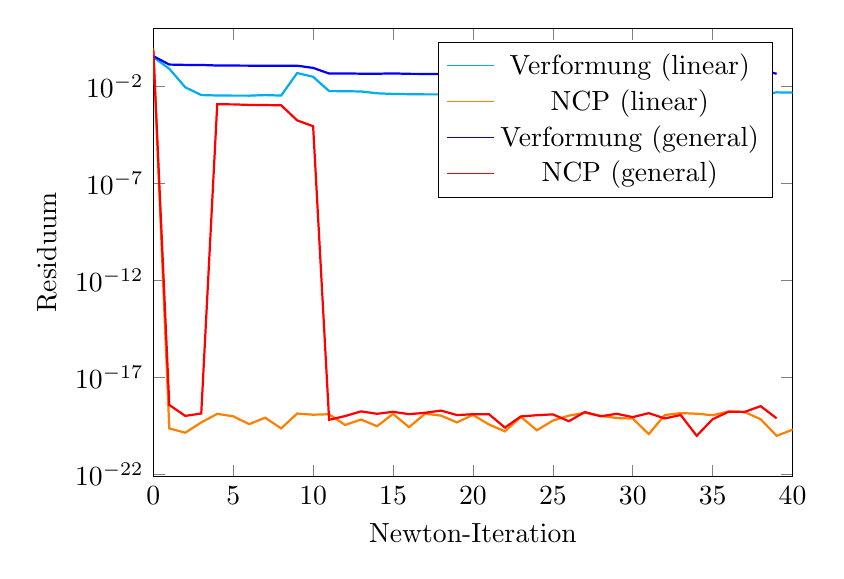
\begin{tikzpicture}[every plot/.append style={thick}] 
\begin{axis}[ 
label style={font=\normalsize}, 
xlabel={Newton-Iteration}, 
ylabel={Residuum}, 
xmin=0, xmax=40, 
ymode=log, 
ymin=0, ymax=10, 
width=0.8\textwidth, 
height=0.6\textwidth, 
legend pos=north east, 
legend style={cells={align=left}}, 
grid style=dashed, 
] 
\addplot[ 
color=cyan, 
] 
coordinates { 
(0, 3.24e-01)(1, 8.17e-02)(2, 9.03e-03)(3, 3.61e-03)(4, 3.42e-03)(5, 3.37e-03)(6, 3.36e-03)(7, 3.59e-03)(8, 3.39e-03)(9, 4.91e-02)(10, 3.15e-02)(11, 5.78e-03)(12, 5.68e-03)(13, 5.51e-03)(14, 4.44e-03)(15, 4.11e-03)(16, 4.00e-03)(17, 3.91e-03)(18, 3.91e-03)(19, 3.89e-03)(20, 4.58e-03)(21, 3.82e-03)(22, 3.73e-03)(23, 3.74e-03)(24, 3.93e-03)(25, 3.76e-03)(26, 3.67e-03)(27, 3.66e-03)(28, 3.66e-03)(29, 4.28e-03)(30, 4.24e-03)(31, 4.15e-03)(32, 3.98e-03)(33, 3.80e-03)(34, 3.61e-03)(35, 3.68e-03)(36, 3.66e-03)(37, 3.62e-03)(38, 3.61e-03)(39, 4.97e-03)(40, 4.81e-03)(41, 5.37e-03)(42, 4.87e-03)(43, 5.08e-03)(44, 4.39e-03)(45, 4.15e-03)(46, 4.17e-03)(47, 4.25e-03)(48, 4.16e-03)(49, 3.81e-03)(50, 3.65e-03)(51, 3.63e-03)(52, 3.62e-03)}; 
\addlegendentry{Verformung (linear)} 
\addplot[ 
color=orange, 
] 
coordinates { 
(0, 9.27e-01)(1, 2.40e-20)(2, 1.44e-20)(3, 4.89e-20)(4, 1.35e-19)(5, 1.01e-19)(6, 3.97e-20)(7, 8.57e-20)(8, 2.40e-20)(9, 1.40e-19)(10, 1.22e-19)(11, 1.29e-19)(12, 3.60e-20)(13, 6.91e-20)(14, 3.12e-20)(15, 1.35e-19)(16, 2.79e-20)(17, 1.36e-19)(18, 1.10e-19)(19, 4.89e-20)(20, 1.20e-19)(21, 3.83e-20)(22, 1.69e-20)(23, 9.44e-20)(24, 1.92e-20)(25, 6.06e-20)(26, 1.09e-19)(27, 1.53e-19)(28, 1.07e-19)(29, 8.19e-20)(30, 7.73e-20)(31, 1.22e-20)(32, 1.17e-19)(33, 1.48e-19)(34, 1.37e-19)(35, 1.15e-19)(36, 1.79e-19)(37, 1.68e-19)(38, 7.18e-20)(39, 1.00e-20)(40, 2.06e-20)(41, 9.37e-20)(42, 9.04e-20)(43, 8.62e-20)(44, 1.23e-19)(45, 1.48e-19)(46, 6.78e-20)(47, 1.27e-19)(48, 1.51e-19)(49, 1.15e-19)(50, 1.92e-20)(51, 1.27e-19)(52, 1.12e-19)}; 
\addlegendentry{NCP (linear)} 
\addplot[ 
color=blue, 
] 
coordinates { 
(0, 3.65e-01)(1, 1.34e-01)(2, 1.29e-01)(3, 1.28e-01)(4, 1.20e-01)(5, 1.19e-01)(6, 1.18e-01)(7, 1.17e-01)(8, 1.17e-01)(9, 1.17e-01)(10, 9.05e-02)(11, 4.62e-02)(12, 4.67e-02)(13, 4.55e-02)(14, 4.52e-02)(15, 4.69e-02)(16, 4.46e-02)(17, 4.42e-02)(18, 4.42e-02)(19, 4.39e-02)(20, 5.41e-02)(21, 5.81e-02)(22, 4.56e-02)(23, 4.53e-02)(24, 4.50e-02)(25, 4.51e-02)(26, 4.49e-02)(27, 4.68e-02)(28, 4.58e-02)(29, 4.54e-02)(30, 4.52e-02)(31, 4.51e-02)(32, 4.74e-02)(33, 4.75e-02)(34, 4.51e-02)(35, 6.81e-02)(36, 2.03e-01)(37, 1.86e-01)(38, 7.47e-02)(39, 4.49e-02)}; 
\addlegendentry{Verformung (general)} 
\addplot[ 
color=red, 
] 
coordinates { 
(0, 7.27e-01)(1, 3.88e-19)(2, 1.06e-19)(3, 1.41e-19)(4, 1.21e-03)(5, 1.19e-03)(6, 1.12e-03)(7, 1.10e-03)(8, 1.07e-03)(9, 1.79e-04)(10, 8.94e-05)(11, 6.66e-20)(12, 1.04e-19)(13, 1.81e-19)(14, 1.36e-19)(15, 1.72e-19)(16, 1.30e-19)(17, 1.53e-19)(18, 1.99e-19)(19, 1.17e-19)(20, 1.29e-19)(21, 1.30e-19)(22, 2.65e-20)(23, 9.96e-20)(24, 1.15e-19)(25, 1.27e-19)(26, 5.61e-20)(27, 1.68e-19)(28, 1.01e-19)(29, 1.36e-19)(30, 9.16e-20)(31, 1.47e-19)(32, 7.82e-20)(33, 1.18e-19)(34, 1.00e-20)(35, 7.20e-20)(36, 1.74e-19)(37, 1.70e-19)(38, 3.37e-19)(39, 7.97e-20)}; 
\addlegendentry{NCP (general)} 
\end{axis} 
\end{tikzpicture} 
\caption{Residuen des Stoffgesetzes 'St.Venant' mit Hinderniss 'Hut' und 8450 Freiheitsgraden für die Verschiebung.} 
\label{fiq:St.Venant_Hut_level5} 
\end{figure} 
